\documentclass[11pt]{article}
\usepackage[utf8]{inputenc}
\usepackage{amsfonts}
\usepackage{amsmath} 
\usepackage{hyperref}
\usepackage{amssymb}
\usepackage{amsthm}
\usepackage{tikz}
\usepackage{geometry}
\usepackage{mathtools}

\newtheorem{theorem}{Theorem}[section]
\newtheorem{lemma}[theorem]{Lemma}
\newtheorem{proposition}[theorem]{Proposition}
\newtheorem{corollary}[theorem]{Corollary}


\title{Sample LaTex Document}
\author{Tom Grubb}
\date{January 2021}


\begin{document}

\maketitle

\abstract{Abstract abstract abstract abstract abstract wow what a useful informative abstract.}

\section{Introduction}
This is a very basic LaTex document. It was created for UCSD's Math 157 class to highlight some of LaTex's functionality. The .tex file starts with a \emph{preamble}, which includes details on the title of this document, as well as several import statements. The result of compiling that .tex file is this pdf. This document was created online using Overleaf.

\section{A Theorem, a Proof, and the Align Environment}
In this section we will prove a basic fact about \textbf{natural numbers}. Look at how the phrase natural numbers is \emph{bolded} and how the word bolded is italicized; you can see how this was done in the source file.

\begin{theorem}
For an integer $n,$ $n\geq 1$, we have 
$$
\sum_{k = 1}^{n} k = \frac{n(n+1)}{2}
$$
\end{theorem}

\begin{proof}
We induct on $n$. In the base case, $n=1$. In this case the sum on the left hand side has a single term equal to $1$ in it. The right hand side simplifies to 
$$
\frac{1\cdot 2}{2} = 1.
$$
Thus the base case holds. 

For the induction step, assume the theorem holds for some integer $n$. Then 
$$
\sum_{k=1}^{n+1} = (n+1) + \sum_{k=1}^nk.
$$
By the induction hypothesis, 
$$
\sum_{k=1}^{n}k = \frac{n(n+1)}{2},
$$
and thus 
$$
\sum_{k=1}^{n+1} = (n+1)+ \frac{n(n+1)}{2}.
$$
Simplifying the right hand side gives 
\begin{align*}
\sum_{k=1}^{n+1} &= \frac{2(n+1)+n(n+1)}{2} \\
&=\frac{(n+1)(n+2)}{2}.
\end{align*}
This finishes the proof of our theorem.
\end{proof}

In the next section we will explore other LaTex environments.

\section{LaTex Lists}
In LaTex you can make bulleted and numbered lists. A bulleted list uses the itemize environment:
\begin{itemize}
    \item This is the first entry in a bulleted list.
    \item This is the second entry in a bulleted list.
\end{itemize}
A numbered list uses the enumerate environment:
\begin{enumerate}
    \item This is the first entry in a numbered list.
    \item This is the second entry in a numbered list. It has a sublist in it!
    \begin{enumerate}
        \item This is a sublist within my numbered list! It uses a nested enumerate environment.
        \item Wow!
    \end{enumerate}
\end{enumerate}

\section{LaTex Tables}
There are two ways of making tables in LaTex. The tabular environment is for making \emph{text based tables}. Often you highlight a tabular environment using the \emph{center} environment:
\begin{center}
    \begin{tabular}{c|c}
    The columns are separated by ampersands & This is column 2 \\
    The rows are separated by two backslashes.  & This is row 2, column 2
\end{tabular}
\end{center}
You can add horizontal lines to the table using the hline command. Vertical lines are formed by adding pipes into the table metadata: \{ $\vert$ c $\vert$ c $\vert$\} means you have two columns which are \emph{centrally aligned} and have vertical lines in between each column: 
\begin{center}
    \begin{tabular}{|c|c|}
    \hline
    The columns are separated by ampersands & This is column 2 \\
    \hline
    The rows are separated by two backslashes.  & This is row 2, column 2\\
    \hline
\end{tabular}
\end{center}
You could optionally change the alignment using l, c, or r in the table metadata:
\begin{center}
    \begin{tabular}{|l|c|r|}
    \hline
    Col 1& Col 2& Col3\\
    \hline
    Left aligned & Centrally aligned & Right aligned \\
    \hline
    
\end{tabular}
\end{center}

An array environment is similar to a tabular environment, but it is for math mode/numeric data. In particular, it should go between double dollar signs, or in an equation environment:
\begin{equation}
    \begin{array}{|c|c|}
    \hline
        \pi & \tau \\
        \hline
         3.14\dots&6.28\dots \\
         \hline
    \end{array}
\end{equation}
Note that the equation environment implicitly numbers the equations. You can change this by messing around with the settings if you wanted. 

\section{Tikz}
If you want to get fancy with your files, you can use Tikz to create images/plots within your file. This is more advanced and will not be necessary for this class, but here are some examples that I have taken from Overleaf's documentation (available here: \url{https://www.overleaf.com/learn/latex/TikZ_package}):
\begin{center}
\begin{tikzpicture}

\draw (-2,0) -- (2,0);
\filldraw [gray] (0,0) circle (2pt);
\draw (-2,-2) .. controls (0,0) .. (2,-2);
\draw (-2,2) .. controls (-1,0) and (1,0) .. (2,2);

\end{tikzpicture}

\end{center}

\begin{center}
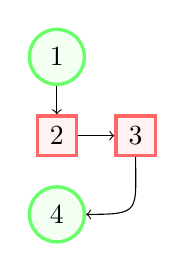
\begin{tikzpicture}[
roundnode/.style={circle, draw=green!60, fill=green!5, very thick, minimum size=7mm},
squarednode/.style={rectangle, draw=red!60, fill=red!5, very thick, minimum size=5mm},
]
%Nodes
\node[squarednode]      (maintopic)                              {2};
\node[roundnode]        (uppercircle)       [above of=maintopic] {1};
\node[squarednode]      (rightsquare)       [right of=maintopic] {3};
\node[roundnode]        (lowercircle)       [below of=maintopic] {4};

%Lines
\draw[->] (uppercircle.south) -- (maintopic.north);
\draw[->] (maintopic.east) -- (rightsquare.west);
\draw[->] (rightsquare.south) .. controls +(down:7mm) and +(right:7mm) .. (lowercircle.east);
\end{tikzpicture}
\end{center}
For more on TikZ, I recommend Google or Office Hours.
\section{Conclusion}
Hopefully this document helps! LaTex is very well documented online, so Googling is always a good way to get more information. But you can always reach out to course staff for a more in depth discussion of LaTex!

\end{document}
